\section{Survival of small populations}
\label{m:sec:small}

Return to the binary process of \cref{m:sec:deathordivision} and suppose it is near
critical, either just below or just above. With the probability of division $p$ and
of death $1-p$ each close to a half, a lineage dies at its first round almost half
the time. Should it survive one generation, both its offspring fail at their own
first attempt with probability around $0.25$, so the lineage reaches the second
generation only with probability about $0.375$:
\begin{equation*}
0.375 \approx
\underbrace{(1-0.5)}_{\text{no extinction at the first step}}\times
\underbrace{(1-0.5\times0.5)}_{\text{nor at the second}} .
\end{equation*}

More generally, survival to a given generation is obtained by iterating the \pgf{}.
With $\phi(z)=pz^2+(1-p)$ from \cref{m:eq:pgfbinary}, the extinction and survival
probabilities follow from
\begin{equation}
\label{m:eq:ext}
u_{n+1} = p\,u_n^2 + 1-p,
\qquad
S_{n+1} = 2pS_n - pS_n^2 ,
\end{equation}
started at $u_0=0$, $S_0=1$. At exactly critical branching this gives, for
$n=1,2,3,4$,
\begin{equation*}
u_n = 0.500,\ 0.625,\ 0.695,\ 0.741\qquad(3\ \text{s.f.}),
\end{equation*}
so the probability of survival decays quickly over the first few rounds of
division, and does so almost as fast just above criticality as just below.
\Cref{m:fig:earlySn} makes the point: whatever advantage supercriticality confers, it
is not an early-generation advantage.

\begin{figure}[ht]
\centering
  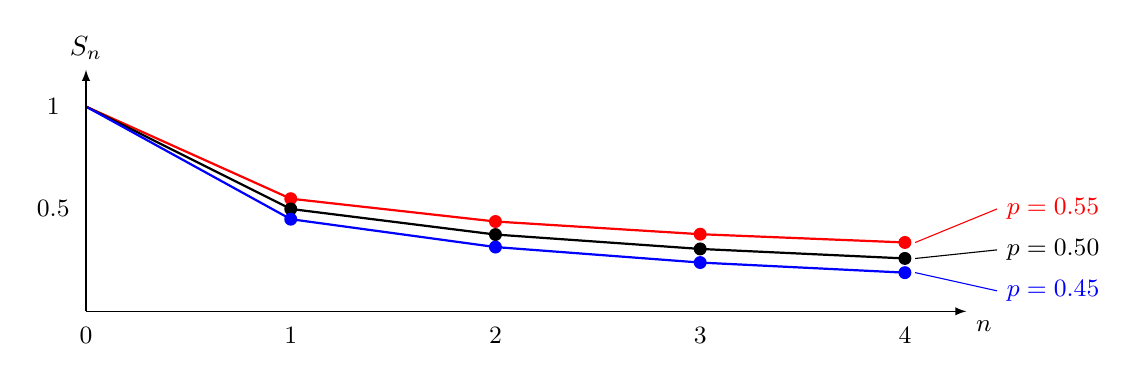
\begin{tikzpicture}[scale = 2.6]
    \foreach \x/\y/\color in {1/0.55/red, 2/0.4386250/red, 3/0.3766719/red, 4/0.336304/red,
                              1/0.5/black, 2/0.375/black, 3/0.3046875/black, 4/0.25827/black,
                              1/0.449999/blue, 2/0.313874/blue, 3/0.2381546/blue, 4/0.188816/blue}
      \fill[color=\color] (\x, \y) circle (0.9pt);
    \draw[red, thick] (0, 1) -- (1, 0.55) -- (2, 0.4386250) -- (3,0.3766719) -- (4,0.336304);
    \draw[black, thick] (0, 1)--(1,0.5) --  (2,0.375) -- (3,0.304687) -- (4,0.25827);
    \draw[blue, thick] (0, 1)--(1,0.449999)  --  (2,0.313874) -- (3,0.238154) -- (4,0.18881);
    \draw[-latex] (0,0) -- (4.3,0) node[below right, font=\small] {$n$};
    \draw[-latex] (0,0) -- (0,1.18) node[above] {$S_n$};
    \foreach \x/\lab in {0/0, 1/1, 2/2, 3/3, 4/4} \node[font=\small] at (\x, -0.12) {\lab};
    \foreach \y/\lab in {0.5/0.5, 1/1} \node[font=\small] at (-0.16, \y) {\lab};
    \draw[red,  thin] (4.05,0.336) -- (4.45,0.50);
    \draw[black,thin] (4.05,0.258) -- (4.45,0.30);
    \draw[blue, thin] (4.05,0.189) -- (4.45,0.10);
    \node[red,  font=\small, anchor=west] at (4.45, 0.50) {$p=0.55$};
    \node[black,font=\small, anchor=west] at (4.45, 0.30) {$p=0.50$};
    \node[blue, font=\small, anchor=west] at (4.45, 0.10) {$p=0.45$};
  \end{tikzpicture}
\caption{Survival probability over the first four generations from a single
progenitor, computed from \cref{m:eq:ext}. Even in the supercritical case
($p=0.55$) the early decay is steep, and the three curves have barely separated by
$n=4$.}
\label{m:fig:earlySn}
\end{figure}

\subsection{An initial cohort of size \texorpdfstring{$k$}{k}}
\label{m:sec:cohort}

Now suppose $Z_0=k$: the process begins not with a single individual but with a
group, small to moderate in number, perhaps $k=10$. Under supercritical branching,
growth becomes more predictably exponential as the count rises, because a large
number of individuals lets the expected dynamics show through the noise of
individual events. The founding cohort is precisely the regime in which that noise
dominates instead.

What, then, are such a cohort's chances of long-run persistence? The question is
answered by asking for the probability that at least one descendant remains, that
is, that not every one of the $k$ founding lineages has died out. The lineages are
independent and each is extinct by generation $n$ with probability $u_n$, so all
$k$ have gone with probability $u_n^{\,k}$, and
\begin{equation}
\label{m:eq:Snk}
S^{(k)}_n = 1-u_n^{\,k} = 1-(1-S_n)^k .
\end{equation}
The identity separates two effects: $S_n$ contains the dynamics of one lineage,
whereas the exponent $k$ contains the founding size. For small $S_n$ one has
$S_n^{(k)}\sim kS_n$ when $kS_n\ll1$, but the exact formula is needed once the
survival chance is no longer small.

\begin{figure}[ht]
\centering
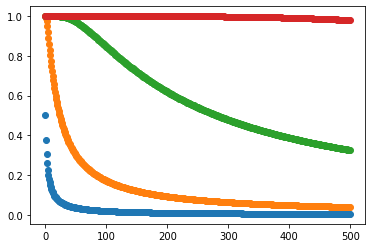
\includegraphics[width=0.56\textwidth]{figures/kvals.png}
\caption{Survival probability $S^{(k)}_n$ from \cref{m:eq:Snk} out to $500$
generations at exact criticality, $p=0.5$, for $k=1,10,100,1000$ (blue through to
red). A larger founding cohort buys longevity, but at criticality every curve is
still headed for zero.}
\label{m:fig:kvals}
\end{figure}

\begin{figure}[ht]
\centering
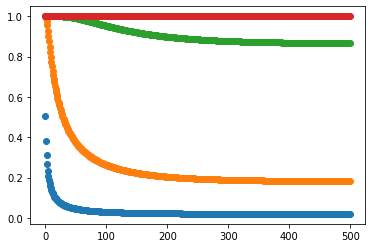
\includegraphics[width=0.45\textwidth]{figures/kvals505.png}
\hfill
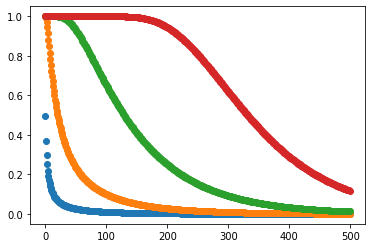
\includegraphics[width=0.45\textwidth]{figures/kvals495.png}
\caption{As \cref{m:fig:kvals}, but with $p$ displaced slightly from criticality:
$p=0.505$ on the left (supercritical), $p=0.495$ on the right (subcritical). The
benefit of a large initial cohort is acutely sensitive to which side of $\tfrac12$
the process sits on. A displacement of half a per cent separates curves that were
nearly coincident in \cref{m:fig:kvals}.}
\label{m:fig:kvals2}
\end{figure}

\Cref{m:fig:kvals,m:fig:kvals2} show $S_n^{(k)}$ through $500$ generations for
$k=1,10,100,1000$. The effect visible in \cref{m:fig:kvals} --- that a larger first
cohort gives improved longevity --- is highly sensitive to criticality. Persistence
improves quickly as $p$ approaches $\tfrac12$ from below and continues to improve
dramatically into supercriticality, and the two panels of \cref{m:fig:kvals2} differ
only in the third decimal place of $p$.

\subsection{Conditioning and apparent early growth}
\label{m:sec:earlyrep}

The conditioning of \cref{m:sec:qsd} has a mirror image which is worth recording,
because it shows that the effect is not confined to the subcritical case.

Consider an ensemble of independent homogeneous birth--death processes, all with
the same constant rates, and retain only those that happen still to be alive at
some large time. The retained subpopulation is automatically enriched for early
rapid growth: a realisation that grew quickly at the outset is far more likely to
have escaped the early extinction risk documented in \cref{m:fig:earlySn}, and so
far more likely to be in the retained set. No change in the underlying rates is
required to produce the enrichment, and the apparent slowdown that follows is not a
slowdown at all but a reversion to the mean. The effect is known as the \emph{push
of the past}, and was identified in a setting far from the present one, as an
explanation for a systematic pattern in longevity and diversity data
\cite{Budd2018}.

That is exactly the conditioning of \cref{m:sec:qsd} seen from the other side. There
a subcritical process was conditioned on survival and its mean settled to $1/A(p)$
rather than decaying; here a critical or supercritical process is conditioned on
survival to a late time and its early growth appears inflated. In both cases the
conditioning, not the mechanism, does the work: selection is being performed on
paths after they have been generated.

The parallel suggests a modelling hypothesis that later chapters take up: that
early replication weighs heavily on eventual survival, even when later per-capita
rates are unchanged. \Cref{m:fig:earlySn} is the reason to take it seriously, since
the first few generations are where nearly all of the extinction risk sits.

\subsection{Discrete birth--death--catastrophe}
\label{m:sec:bdc}

A birth--death process subject to catastrophe carries, alongside the possibility of
extinction by death, the possibility of an abrupt event that removes the population
at a stroke. In discrete time and up to the point of catastrophe such a process
behaves exactly as the basic Galton--Watson model as far as its limiting
conditional distribution is concerned. Conditioning on non-catastrophe, and
conditioning also on non-extinction by death, it exhibits a stationary limiting
distribution. Whether a quasi-stationary distribution survives when one conditions
on \emph{neither} death nor catastrophe is a separate question, and one best
settled by simulation. Either way it is useful to have the probability of
non-catastrophe in hand.

\subsubsection*{Probability of catastrophe at step \texorpdfstring{$n$}{n}}

Let $\kappa$ be the probability that a given individual initiates catastrophe at a
step, and write $c = 1-\kappa$. A single individual fails to do so with probability
$c$, two with $c^2$, and a cohort of size $N$ with $c^N$.

Consider first birth and catastrophe alone, with no death, so $p=1$. Then the
census of the living population at any generation is known with certainty: from a
single progenitor the population simply doubles at each step prior to catastrophe.
Conditional on reaching step $n$, where $2^{n-1}$ individuals are exposed, the
process therefore comes to its abrupt halt at that step with probability
\begin{equation}
\label{m:eq:bdchalt}
h_n = 1-c^{2^{\,n-1}},
\end{equation}
one minus the probability that none of the $2^{n-1}$ individuals present caused it.
This is a \emph{conditional} hazard: it assumes step $n$ is reached. The
unconditional probability that catastrophe first occurs at step $n$ is smaller,
because every earlier step must also have been passed.

\subsubsection*{Probability of process survival}

Still with no death, define $S_n$ as the probability that the process survives to
generation $n$. Survival to generation $0$ is certain, $S_0=1$. Survival to
generation $1$ requires only that the founder divided without catastrophe,
$S_1=c$. Persistence to step $2$ requires that the founder divided and that
each of its two offspring did too, so $S_2 = c\,c^2$. The pattern
is clear: survival to generation $n$ requires every prior step to have been passed,
and therefore
\begin{equation}
\label{m:eq:bdcS}
S_n = \prod_{i=0}^{n-1}c^{2^i}
= c^{\sum_{i=0}^{n-1}2^i}
= c^{2^n-1} .
\end{equation}
The unconditional mass function of the first-catastrophe time follows at once:
\begin{equation}
\label{m:eq:bdcfirst}
\pr[\big]{K = n} = S_n\,h_n = c^{2^n-1}\lrb{1-c^{2^n}} .
\end{equation}
The factor $S_n$ is indispensable; $h_n$ alone is a conditional hazard, not an
exact-time probability, and conflating the two is the standard error of mean-field
hazard reasoning, which substitutes the current expected census into a rate as
though the census were deterministic.

\subsubsection*{Death included}

The difficulty comes once death is allowed, because the size of the living
population is then no longer known with certainty from one generation to the next.
Let $\widetilde Z_i$ denote the underlying binary Galton--Watson population with
the catastrophe mechanism switched off, and write
\begin{equation}
\label{m:eq:Hn}
H_n = \sum_{i=0}^{n-1}\widetilde Z_i
\end{equation}
for the cumulative exposure over the first $n$ steps. Conditioning on the whole
catastrophe-free genealogy gives the exact identity
\begin{equation}
\label{m:eq:noruptureexact}
\pr[\big]{\text{no catastrophe before }n}
= \ex{c^{H_n}} .
\end{equation}
The natural guess is that the probabilities shake out when the expected population
is used in place of the actual one:
\begin{equation}
\label{m:eq:bdcguess}
\ex{c^{H_n}} \overset{?}{=} c^{\sum_{i=0}^{n-1}\ex{\widetilde Z_i}} .
\end{equation}
This is a heuristic substitution and not an identity; the direction of the error
can be pinned down exactly. The map $N\mapsto c^N$ is convex, so Jensen's
inequality gives $\ex{c^{\widetilde Z_i}}\ge c^{\ex{\widetilde Z_i}}$: replacing
the random census by its mean systematically understates the chance of getting
through a step. With $m=2p$,
\begin{equation}
\label{m:eq:meanexposure}
\ex{H_n} = \sum_{i=0}^{n-1}m^i
= \begin{cases}
\dfrac{1-m^n}{1-m}, & m\neq1,\\[2mm]
n, & m=1,
\end{cases}
\end{equation}
and \cref{m:eq:bdcguess} is better read as the lower bound
$\pr[\big]{\text{no catastrophe before }n}\ge c^{\ex{H_n}}$ than as an equality.
Nor are the steps independent, since surviving one is evidence of a smaller
population, which raises the chance of surviving the next; both effects push the
same way. How tight a bound remains a question for numerical work.

Non-rupture should not be confused with population survival. If the requirement is
that the population be both unruptured and non-zero at generation $n$, the exact
probability is
\begin{equation}
\label{m:eq:jointsurvival}
\ex{\ind_{\{\widetilde Z_n>0\}}\,c^{H_n}},
\end{equation}
for which the Jensen bound does not directly provide an estimate. The distinction
removes an ambiguity in the elementary approximation and indicates why the joint
quasi-stationary problem is better posed through the killed-chain generator
developed below.

The process can nevertheless be described exactly by a weighted generating
function. Define
\begin{equation}
\label{m:eq:catweightedpgf}
F_n(s) = \ex{s^{\widetilde Z_n}\,c^{H_n}},
\qquad F_0(s) = s .
\end{equation}
Conditioning on the founder's reproduction --- death with probability $1-p$, or
division with probability $p$, after which two independent subtrees each contribute
a factor $F_n$ and the founder's own step contributes $c$ --- gives the closed
recursion
\begin{equation}
\label{m:eq:catweightedrec}
F_{n+1}(s) = c\,\phi\bigl(F_n(s)\bigr)
= c\lrb{1-p+pF_n(s)^2} .
\end{equation}
Its evaluations at special points have distinct meanings: $F_n(1)$ is the
probability of no catastrophe in the first $n$ updates, agreeing with
\cref{m:eq:noruptureexact}, while $F_n(1)-F_n(0)$ is the probability of being both
unruptured and non-extinct at generation $n$, the quantity of
\cref{m:eq:jointsurvival}. The recursion \cref{m:eq:catweightedrec} is exact, and
it is the natural object to iterate when the Jensen bound is too crude.

\subsection{Continuous-time birth--death}
\label{m:sec:cts}

The discrete constant $A(p)$ of \cref{m:sec:qsd} resists closed-form evaluation,
and \ChA{} is devoted to the analysis that establishes this and to the exact
product, series and asymptotic descriptions that replace a closed form. The
continuous-time counterpart of the process is different: its quasi-stationary
constant \emph{is} elementary, and because the comparison between the two
constants organises much of what follows, the continuous-time calculation is set
out here in full.

Take the linear birth--death process of \cref{m:sec:linbd}, with per-capita birth
rate $\lambda$ and death rate $\mu$, started from $N$ individuals. Its extinction
probability $p_0(t)$ is \cref{m:eq:p0t}, and its survival probability is
$S^{(N)}(t) = 1-p_0(t)$.

\subsubsection*{Limiting mean conditioned on non-extinction}

The process has a stationary conditional mean when $\mu>\lambda$, that is in the
subcritical case. Exactly as in \cref{m:sec:condmean},
\begin{equation}
\label{m:eq:condit}
\ex{X_t\mid X_t>0} = \frac{\ex{X_t}}{S^{(N)}(t)},
\end{equation}
and the late-time limit follows on applying L'H\^opital's rule. It is quicker to
take $N=1$ and compute directly. With $\ex{X_t}=\ee^{(\lambda-\mu)t}$ from
\cref{m:eq:bdmean} and
\begin{equation*}
S(t) = 1-\frac{\mu-\mu\ee^{(\mu-\lambda)t}}{\lambda-\mu\ee^{(\mu-\lambda)t}}
= \frac{\lambda-\mu}{\lambda-\mu\ee^{(\mu-\lambda)t}},
\end{equation*}
\cref{m:eq:condit} gives
\begin{equation*}
\ex{X_t\mid X_t>0} = \frac{\lambda\ee^{(\lambda-\mu)t}-\mu}{\lambda-\mu} .
\end{equation*}
For $\mu>\lambda$ the exponential decays, and the limiting conditional mean is the
constant
\begin{equation}
\label{m:eq:ctsqsmean}
\lim_{t\to\infty}\ex{X_t\mid X_t>0} = \frac{\mu}{\mu-\lambda}
= \frac{1}{1-\lambda/\mu}
\;\lrb{=\frac{1}{\Ac}} .
\end{equation}
At criticality, $\lambda=\mu$, the same quotient gives the exact conditional mean
$\ex{X_t\mid X_t>0} = 1+\lambda t$, which grows without bound: there is no
stationary conditional law at the critical point, in keeping with the discrete
case.

To compare \cref{m:eq:ctsqsmean} with the discrete-time constant the two
parametrisations must be matched, and \cref{m:prop:race} is what matches them: with
birth and death clocks running at rates $\lambda$ and $\mu$, the probability that
the birth clock wins is $p = \lambda/(\lambda+\mu)$, so that
$\lambda/\mu = p/(1-p)$. In that parametrisation
\begin{equation}
\label{m:eq:Acts}
\frac{1}{\Ac} = \frac{1-p}{1-2p},
\qquad\text{that is}\qquad
\Ac(p) = \frac{1-2p}{1-p} ,
\end{equation}
the subscript marking this as the continuous-time constant, to distinguish it from
the discrete-time $A(p)$ of \cref{m:eq:lateS}. Unlike its discrete counterpart,
$\Ac(p)$ is an elementary function of $p$.

\begin{figure}[ht]
\centering

\includegraphics[width=0.5\textwidth]{figures/dtctA.png}
\caption{The continuous-time constant $\Ac(p) = (1-2p)/(1-p)$ (green) against
high-precision numerical values of the discrete-time constant $A(p)$ (red points).
Both vanish at $p=\tfrac12$, but at $p=0$ the continuous curve starts at $1$ and
the discrete one at $\tfrac12$, and the two are not related by a constant factor in
between. The black line is one of the fitted surrogates produced by the
closed-form search recorded in \ChA; it tracks the points closely but is not
exact. The discrepancy between the two constants is resolved in \ChA, where the
lower bound $A(p)>\tfrac12\Ac(p)$ is proved and shown to be attained only in the
limit $p\to0$.}
\label{m:fig:dtct}
\end{figure}

\Cref{m:fig:dtct} plots $\Ac(p)$ against numerically obtained values of $A(p)$,
and raises an obvious question: why does the continuous curve start at $1$ and the
discrete one at $\tfrac12$? Merely halving $\Ac$ does not superpose them, because
at the other end of the range they meet. The complete answer is given in \ChA{}
once the exact series for $A(p)$ is in place; it turns out that $\Ac(p)/2$ is a
strict lower bound for $A(p)$, attained only in the limit $p\to0$, while near
criticality the two constants share the same leading behaviour.

\subsection{Continuous-time birth--death--catastrophe}
\label{m:sec:ctbdc}

The discrete process of \cref{m:sec:bdc} has a continuous-time counterpart, and
since it is the central object of several later chapters it is defined here, in the
notation established above. No results about it are derived in this chapter.

\begin{definition}[Birth--death--catastrophe process]
\label{m:def:bdc}
Let $X_t$ count individuals in a compartment. Each individual independently gives
birth at rate $\lambda$ and dies at rate $\mu$, and the compartment additionally
undergoes a catastrophe --- a rupture that removes the entire population at once
--- at a rate $\rho$ per individual, so that the total catastrophe rate in state
$n$ is $\rho n$. Writing $\dagger$ for the post-catastrophe state, the non-zero
transition rates out of $n\ge1$ are
\begin{equation}
\label{m:eq:bdcrates}
q_{n,n+1} = \lambda n,
\qquad
q_{n,n-1} = \mu n,
\qquad
q_{n,\dagger} = \rho n ,
\end{equation}
and both $n=0$ and $\dagger$ are absorbing.
\end{definition}

Two features distinguish \cref{m:def:bdc} from the linear birth--death process of
\cref{m:sec:linbd}, and both matter later. The process now has \emph{two} absorbing
states, reached by mechanisms that are distinguishable and not interchangeable:
extinction empties the compartment gradually, catastrophe empties it in one event
and releases its contents. And the catastrophe rate is proportional to the
population, so the compartment becomes more likely to rupture the fuller it is.

The generating-function machinery of \cref{m:sec:pgf} applies unchanged. Restricting
attention to realisations that have not yet ruptured and writing
$G(z,t) = \ex{z^{X_t}\ind\{X_t\neq\dagger\}}$, the master equation for
\cref{m:eq:bdcrates} yields
\begin{equation}
\label{m:eq:bdcpde}
\pddt{G} = \bigl(\lambda z^2-(\lambda+\mu+\rho)z+\mu\bigr)\pdd{G}{z},
\qquad G(z,0) = z^{N},
\end{equation}
which differs from \cref{m:eq:bdpde} only in the coefficient of $z$. The quadratic
no longer factorises with a root at $z=1$, and that single change is responsible
for most of what is interesting about the process: probability is not conserved on
the non-ruptured states, and $G(1,t)$ is the survival probability rather than one.

\subsubsection*{The killed-chain viewpoint}

Later chapters analyse processes of this kind through the generator restricted to
the living states, and it is useful to fix the language now. Allow general
state-dependent rates for the moment: from state $i\ge1$, birth at rate
$\lambda_i$, ordinary death at rate $\mu_i$, and catastrophe at rate $\kappa_i$,
with both absorbing outcomes lumped into a single cemetery state. On bounded test
functions the generator is
\begin{multline*}
(\mathcal Lf)(i)
= \lambda_i\{f(i+1)-f(i)\} + \mu_i\{f(i-1)-f(i)\}
+ \kappa_i\{f(0)-f(i)\},
\qquad i\ge1,
\end{multline*}
with $(\mathcal Lf)(0)=0$. Linear birth--death with per-capita catastrophe
corresponds to $\lambda_i=i\lambda$, $\mu_i=i\mu$, $\kappa_i=i\rho$, recovering
\cref{m:def:bdc} once the cemetery is split into extinction and rupture.

Restricting $\mathcal L$ to the positive states gives the \emph{killed
subgenerator} $K$, with
\begin{equation*}
K_{i,i+1}=\lambda_i,\qquad K_{i,i-1}=\mu_i\quad(i\ge2),
\qquad
K_{i,i}=-(\lambda_i+\mu_i+\kappa_i) .
\end{equation*}
The missing row mass is exactly the instantaneous absorption rate: $\kappa_i$ for
$i\ge2$, and $\mu_1+\kappa_1$ for $i=1$, since from a single individual ordinary
death is also absorption. Writing $T_0=\inf\{t\ge0:X_t=0\}$ and summing the
positive-state forward equations gives the survival-loss balance
\begin{equation}
\label{m:eq:survivalloss}
\dda{}{t}\pr{T_0>t}
= -\mu_1\pr{X_t=1} - \sum_{i\ge1}\kappa_i\pr{X_t=i},
\end{equation}
where ordinary death removes survival mass only from state $1$, while catastrophe
can remove it from every positive state.

The balance sharpens the connection with quasi-stationarity. If a distribution
$\nu=(\nu_i)_{i\ge1}$ on the positive states is quasi-stationary and the relevant
sums are finite, then for some $\theta>0$,
\begin{equation}
\label{m:eq:qsdeigen}
\nu K = -\theta\,\nu,
\qquad
\pr[\big]{_\nu}{T_0>t} = \ee^{-\theta t} .
\end{equation}
Indeed, quasi-stationarity writes the unnormalised positive-state law as
$a(t)\nu$; the semigroup property forces $a(s+t)=a(s)a(t)$, and right-continuity
gives $a(t)=\ee^{-\theta t}$; differentiating at zero yields the left-eigenvector
relation. Summing its coordinates and comparing with \cref{m:eq:survivalloss}
identifies the decay rate as
\begin{equation}
\label{m:eq:thetarate}
\theta = \mu_1\nu_1 + \sum_{i\ge1}\kappa_i\nu_i .
\end{equation}

One limiting case is worth isolating. If the catastrophe clock is constant,
$\kappa_i\equiv\kappa$ on the positive states, it may be taken independent of the
underlying birth--death process, and the killed semigroup factorises as
\begin{equation*}
P_t^{K} = \ee^{-\kappa t}\,P_t^{\mathrm{BD},K} .
\end{equation*}
The extra clock shifts the survival decay rate by $\kappa$ but leaves the law
conditional on survival unchanged. A state-dependent sequence such as
$\kappa_i=i\rho$, by contrast, weights paths according to their accumulated
population exposure and generally changes the quasi-stationary law itself. Rates,
means and variances, state probabilities and the associated generating-function
equations for \cref{m:def:bdc} are developed \fwd{bdc}{in the later chapters on
birth--death--catastrophe processes}, with the two-type extension treated
\fwd{multitype}{in the chapter on multi-type processes} and the release of a
ruptured compartment's contents into a shared medium \fwd{rupture}{in the chapter
on compartment rupture}. The method used to solve \cref{m:eq:bdcpde} and its
relatives is the subject of \cref{m:sec:moc}.

\FloatBarrier
